\documentclass[]{article}
\usepackage{lmodern}
\usepackage[compact]{titlesec}
\usepackage{amssymb,amsmath}
\usepackage{ifxetex,ifluatex}
\usepackage{fixltx2e} % provides \textsubscript
\ifnum 0\ifxetex 1\fi\ifluatex 1\fi=0 % if pdftex
  \usepackage[T1]{fontenc}
  \usepackage[utf8]{inputenc}
\else % if luatex or xelatex
  \ifxetex
    \usepackage{mathspec}
  \else
    \usepackage{fontspec}
  \fi
  \defaultfontfeatures{Ligatures=TeX,Scale=MatchLowercase}
\fi
% use upquote if available, for straight quotes in verbatim environments
\IfFileExists{upquote.sty}{\usepackage{upquote}}{}
% use microtype if available
\IfFileExists{microtype.sty}{%
\usepackage{microtype}
\UseMicrotypeSet[protrusion]{basicmath} % disable protrusion for tt fonts
}{}
\usepackage[margin=1in]{geometry}
\usepackage{hyperref}
\hypersetup{unicode=true,
            pdftitle={Visualizing Time},
            pdfauthor={Darryl Buswell},
            pdfborder={0 0 0},
            breaklinks=true}
\urlstyle{same}  % don't use monospace font for urls
\usepackage{graphicx,grffile}
\makeatletter
\def\maxwidth{\ifdim\Gin@nat@width>\linewidth\linewidth\else\Gin@nat@width\fi}
\def\maxheight{\ifdim\Gin@nat@height>\textheight\textheight\else\Gin@nat@height\fi}
\makeatother
% Scale images if necessary, so that they will not overflow the page
% margins by default, and it is still possible to overwrite the defaults
% using explicit options in \includegraphics[width, height, ...]{}
\setkeys{Gin}{width=\maxwidth,height=\maxheight,keepaspectratio}
\IfFileExists{parskip.sty}{%
\usepackage{parskip}
}{% else
\setlength{\parindent}{0pt}
\setlength{\parskip}{6pt plus 2pt minus 1pt}
}
\setlength{\emergencystretch}{3em}  % prevent overfull lines
\providecommand{\tightlist}{%
  \setlength{\itemsep}{0pt}\setlength{\parskip}{0pt}}
\setcounter{secnumdepth}{0}
% Redefines (sub)paragraphs to behave more like sections
\ifx\paragraph\undefined\else
\let\oldparagraph\paragraph
\renewcommand{\paragraph}[1]{\oldparagraph{#1}\mbox{}}
\fi
\ifx\subparagraph\undefined\else
\let\oldsubparagraph\subparagraph
\renewcommand{\subparagraph}[1]{\oldsubparagraph{#1}\mbox{}}
\fi

%%% Use protect on footnotes to avoid problems with footnotes in titles
\let\rmarkdownfootnote\footnote%
\def\footnote{\protect\rmarkdownfootnote}

%%% Change title format to be more compact
\usepackage{titling}

% Create subtitle command for use in maketitle
\newcommand{\subtitle}[1]{
  \posttitle{
    \begin{center}\large#1\end{center}
    }
}

\setlength{\droptitle}{-2em}
  \title{Visualizing Time}
  \pretitle{\vspace{\droptitle}\centering\huge}
  \posttitle{\par}
\subtitle{MSPA PREDICT 455-DL-SEC55}
  \author{Darryl Buswell}
  \preauthor{\centering\large\emph}
  \postauthor{\par}
  \date{}
  \predate{}\postdate{}

\begin{document}
\maketitle

\newpage

\section{1 Introduction}\label{introduction}

This assignment explores trends in demand and supply for sources of
energy, with a particular focus on the U.S. crude oil market. All
datasets presented as part of this assessment have been obtained from
the U.S. Energy Information Agency (Agency 2016), with each in
timeseries format with either an annual or weekly frequency.

\section{2 Data Exploration}\label{data-exploration}

Figure A1 shows a stacked barplot of total energy output according to
source of production within the U.S., from 1950 through to 2015. As the
plot shows, total energy production in the U.S. over all sources saw a
rapid increase from 1950 through to 1970, and then moderate growth
between 1970 and 2005. Since 2005 however, U.S. energy production has
seen another sharp rise. The plot also indicates the major sources of
energy production, with natural gas, crude oil and coal being the major
contributors to total energy production.

We are able to index each of the major sources of production from 2005
in order to track the contribution by source of energy over the 2005 to
2015 period. As shown in Figure A2, we can see that coal energy
production has actually fallen since 2005, which may be partially
attributed to lower demand for coal as countries move towards cleaner
energy sources (Saunders 2015). In contrast, production of crude oil and
natural gas sources has increased. Clearly the rapid rise in total U.S.
energy production between 2005 and 2015 can be mainly attributed to
crude oil and natural gas.

The Organization of the Petroleum Exporting Countries (OPEC) is also a
major producer of crude oil energy products. As Figure A3 shows, OPEC
has not sacrificed any market share over this period of growth in U.S.
petroleum production. In fact, OPEC has also seen a steady increase in
crude oil production from 2005 through to 2015. We can also note the
major OPEC producers, with Saudi Arabia clearly being the dominant
contributor to total OPEC production.

On the demand side, we can see from Figure A4 that while total energy
consumption in the U.S. has increased steadily from 1950 through to
2005, consumption has remained flat since 2005. We can also note that
the Industrial and Transportation sectors have remained the dominant
energy consumers within the U.S. since 1950. Figure A5 reaffirms this
with demand for petroleum products by the wider Organization for
Economic Cooperation and Development (OECD) members actually falling
since 2005. This fall in demand was most notable in France and in the
general category of `Other Members', which includes countries such as
Australia, the United Kingdom and Italy.

With crude oil production growing in the U.S. since 2005 and lackluster
demand for petroleum products from the wider OECD, the effect has been a
fall in U.S. crude oil prices. This can be seen in Figure A6. The sudden
fall in prices over late 2014/early 2015 was, in part, a response to
OPEC's decision to not sacrifice market share to growing U.S. production
(J. Baffes 2015). These factors have contributed to the domestic price
of U.S. Crude Oil falling to prices not seen since the Global Financial
Crisis in 2008.

Figure A7 takes a closer look at crude oil price and supply from the
U.S. over 2015. We note that while oil prices have continued to follow a
downward trend over 2015, crude oil supply out of the U.S. has remained
firm. It may be assumed that the U.S. have chosen not to cut oil supply
to prevent loss of market share to the OPEC and other competitors.

In order to predict U.S. crude oil price, there are a number of options
available. We can apply a simple moving average, a weighted moving
average, specify a linear or non-linear function to the data, or even
apply an Autoregressive Integrated Moving Average (ARIMA) model. Each
option would remain naive to the supply and demand data previously
demonstrated, but provide a simple means for timeseries forecasting.
Prior to fitting a model to the price data, we can decompose the weekly
price series in order to identify underlying seasonality or trend within
the dataset.

Figure A8 shows the decomposed series with a timeseries frequency of 52
weeks. The seasonal effect between years is immediately obvious, with
the decomposition able to isolate a reoccurring seasonal pattern which
explains almost US\$10/barrel of price variance within any given year.
The underlying trend within the data is also presented, providing a more
clear indication of the recent price weakness.

Finally, we fit an ARIMA model to the data in order to generate and
visually represent a forecast of crude oil prices. This model suggests
that prices will continue to fall during 2016.

\section{3 Conclusion}\label{conclusion}

Crude oil production in the U.S. increased dramatically between 2005 and
2015. This increase in production occurred at a time where OPEC members
also increased crude oil production and total demand for petroleum
products either remained flat or declined in many developed economies.
The excess supply relative to demand has led to crude oil prices falling
between 2005 and 2015 to levels not seen since the Global Financial
Crisis. A decomposition of weekly crude oil prices was also plotted.
This plot showed that seasonal patterns account for almost US\$10/barrel
of price variance within any given year.

\section{Appendix A Figure Output}\label{appendix-a-figure-output}

\subsection{Figure A1 U.S. Primiary Energy Production by
Source}\label{figure-a1-u.s.-primiary-energy-production-by-source}

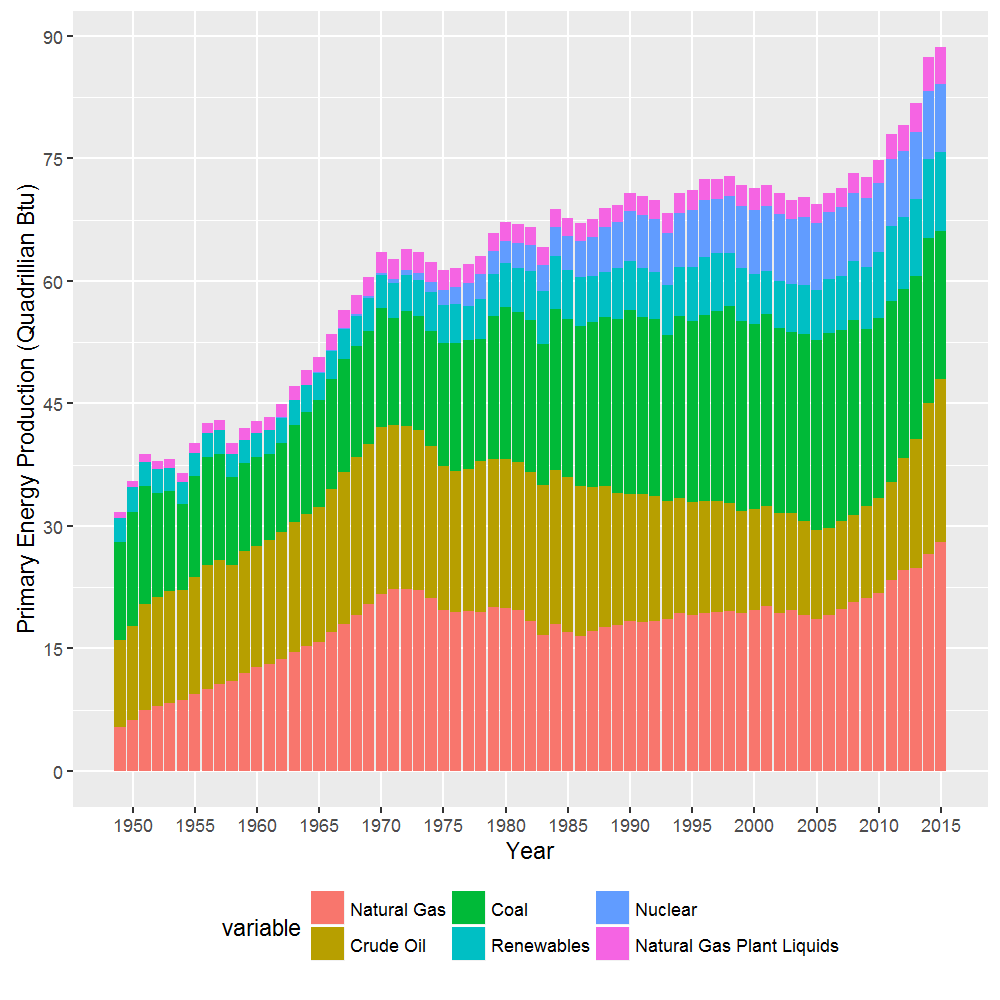
\includegraphics[height=8.33333in]{images/EIAdata_us_primenrg_prod.png}

\newpage

\subsection{Figure A2 U.S. Primiary Energy Production by
Source}\label{figure-a2-u.s.-primiary-energy-production-by-source}

\subsubsection{(indexed to 100x10\^{}15 Btu at
2005)}\label{indexed-to-100x1015-btu-at-2005}

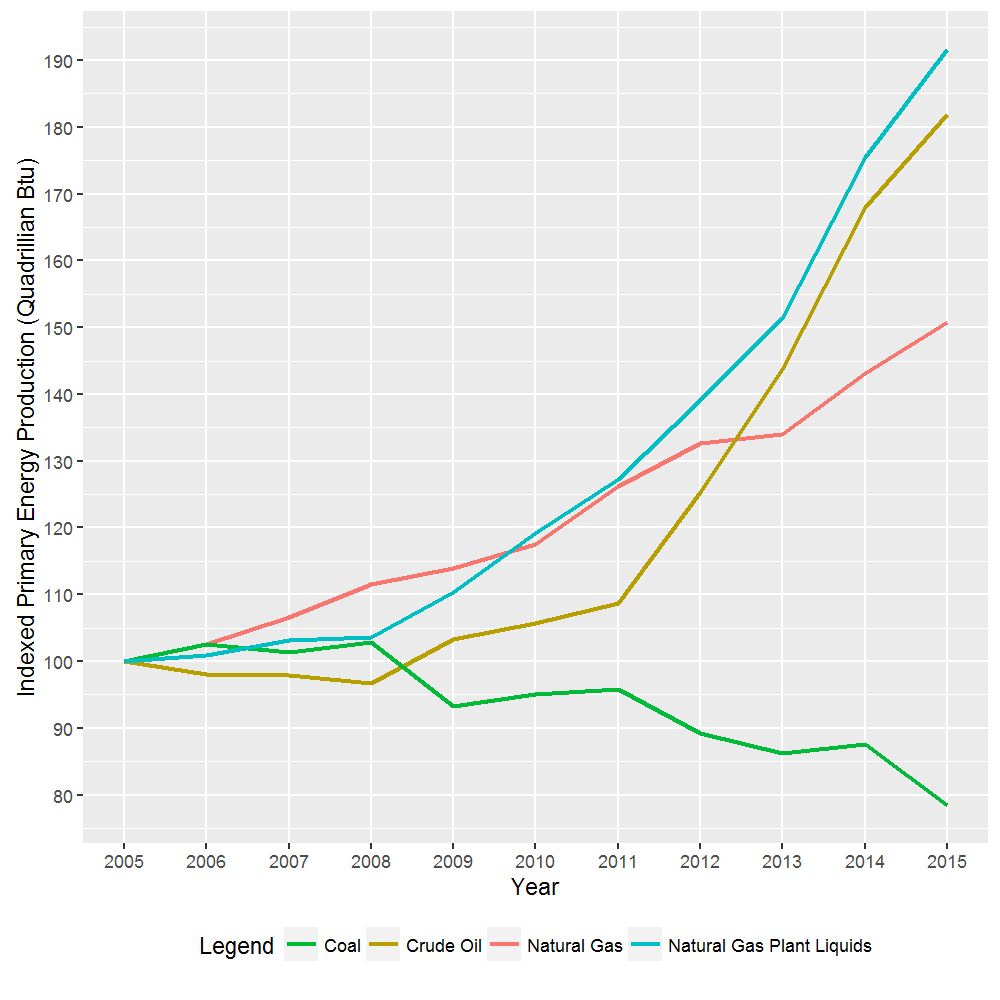
\includegraphics[height=10.41667in]{images/EIAdata_us_primenrg_prod_indexed.png}

\newpage

\subsection{Figure A3 OPEC Crude Oil
Production}\label{figure-a3-opec-crude-oil-production}

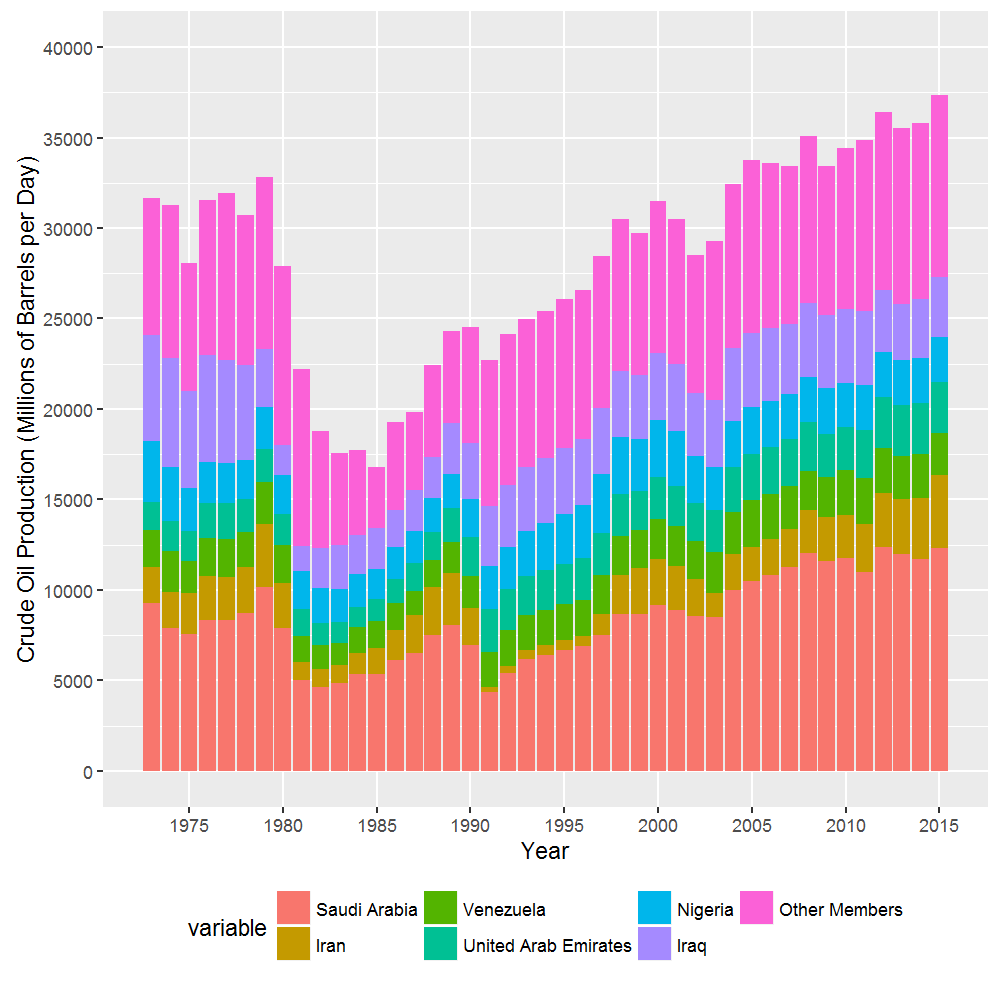
\includegraphics[height=8.33333in]{images/EIAdata_opec_crudeoil_prod.png}

\newpage

\subsection{Figure A4 U.S. Total Energy Consumption by
Industry}\label{figure-a4-u.s.-total-energy-consumption-by-industry}

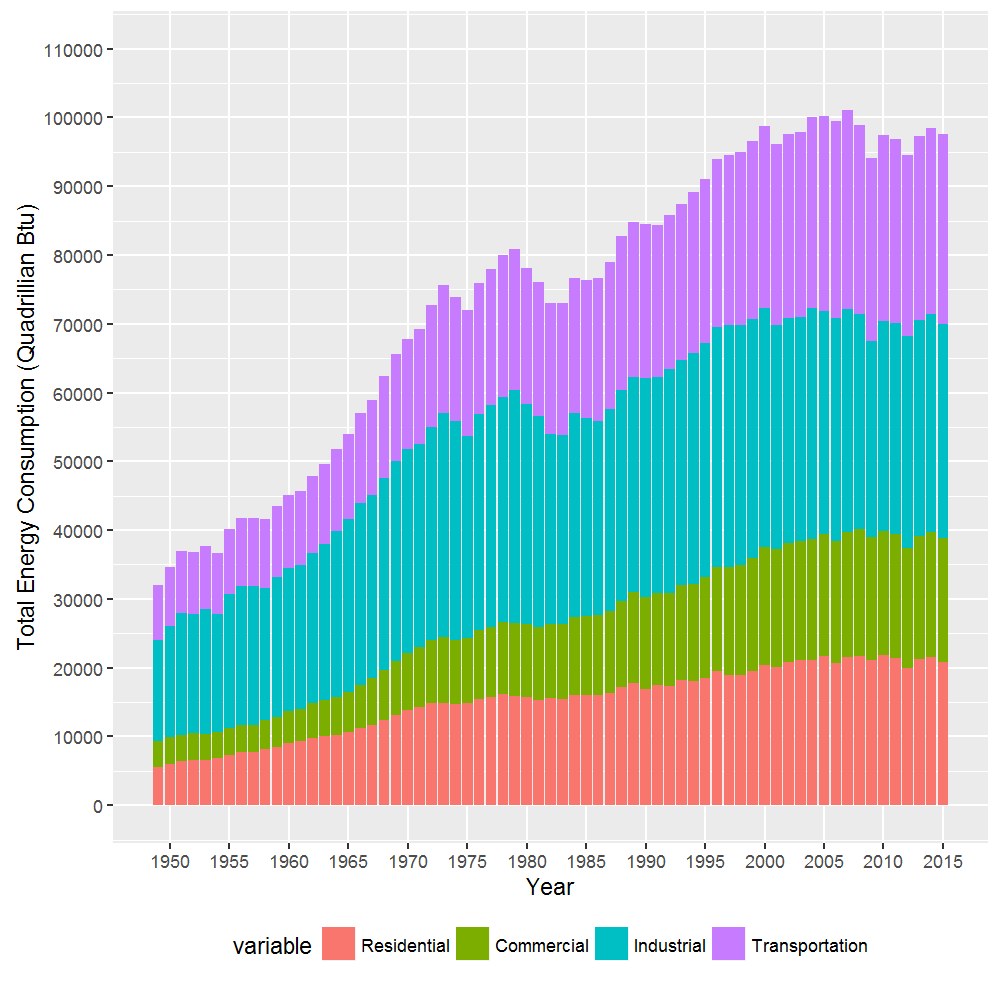
\includegraphics[height=10.41667in]{images/EIAdata_us_totalenrg_cons.png}

\newpage

\subsection{Figure A5 OECD Total Petroleum
Consumption}\label{figure-a5-oecd-total-petroleum-consumption}

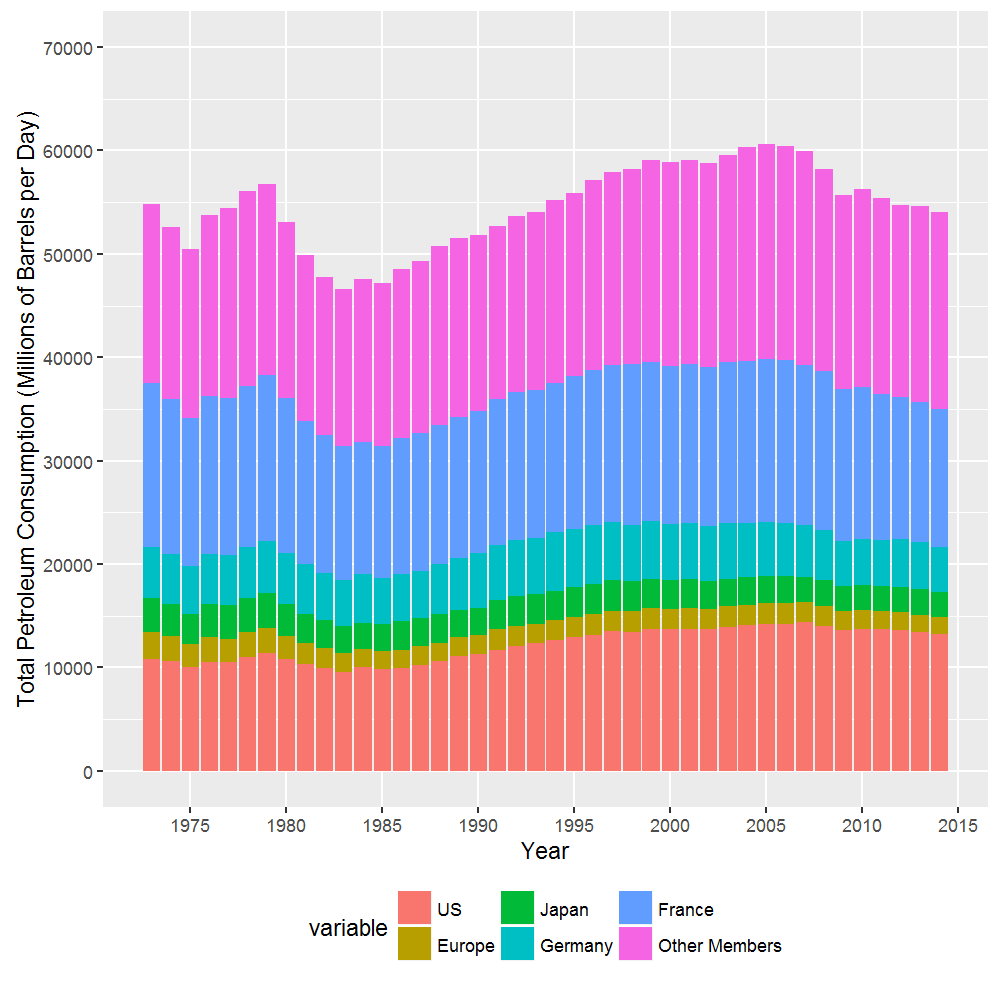
\includegraphics[height=10.41667in]{images/EIAdata_oecd_petrol_cons.png}

\newpage

\subsection{Figure A6 U.S. Crude Oil
Price}\label{figure-a6-u.s.-crude-oil-price}

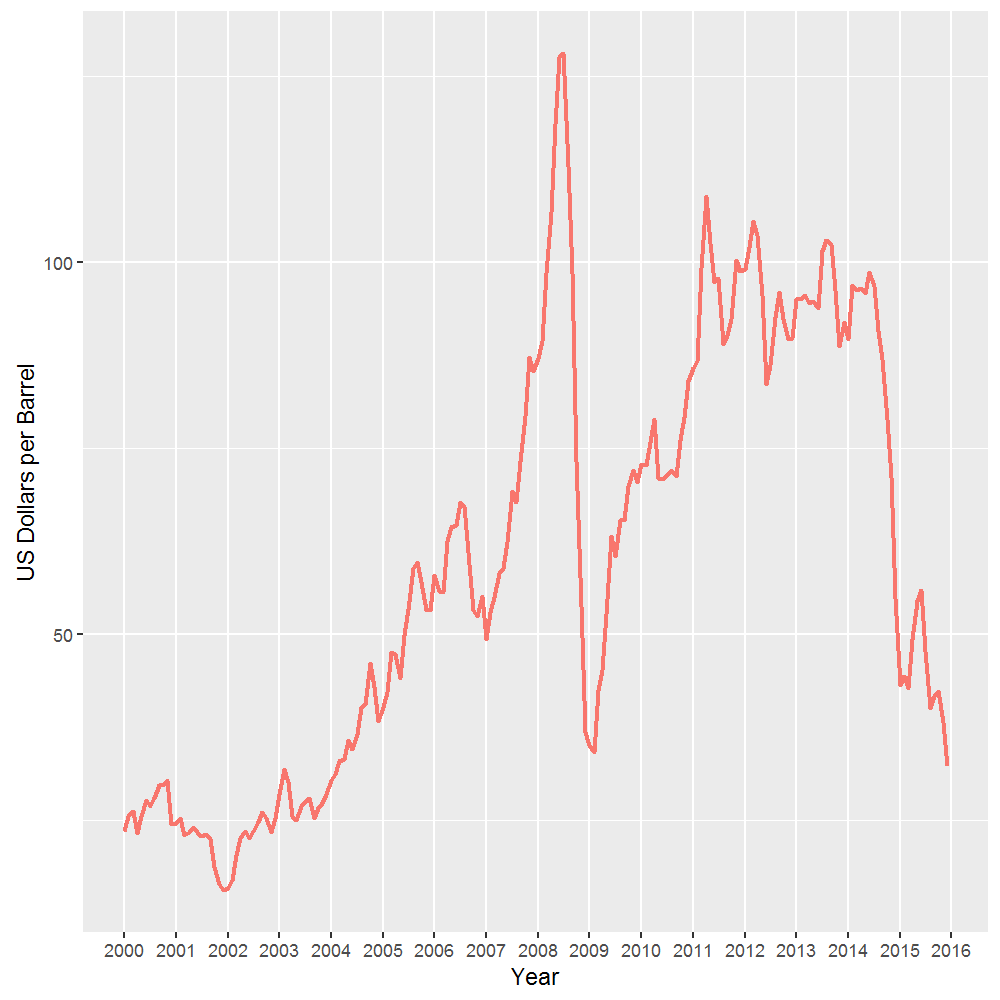
\includegraphics[height=8.33333in]{images/EIAdata_us_crudeoil_price.png}

\newpage

\subsection{Figure A7 U.S. Crude Oil Price versus U.S. Crude Oil
Supply}\label{figure-a7-u.s.-crude-oil-price-versus-u.s.-crude-oil-supply}

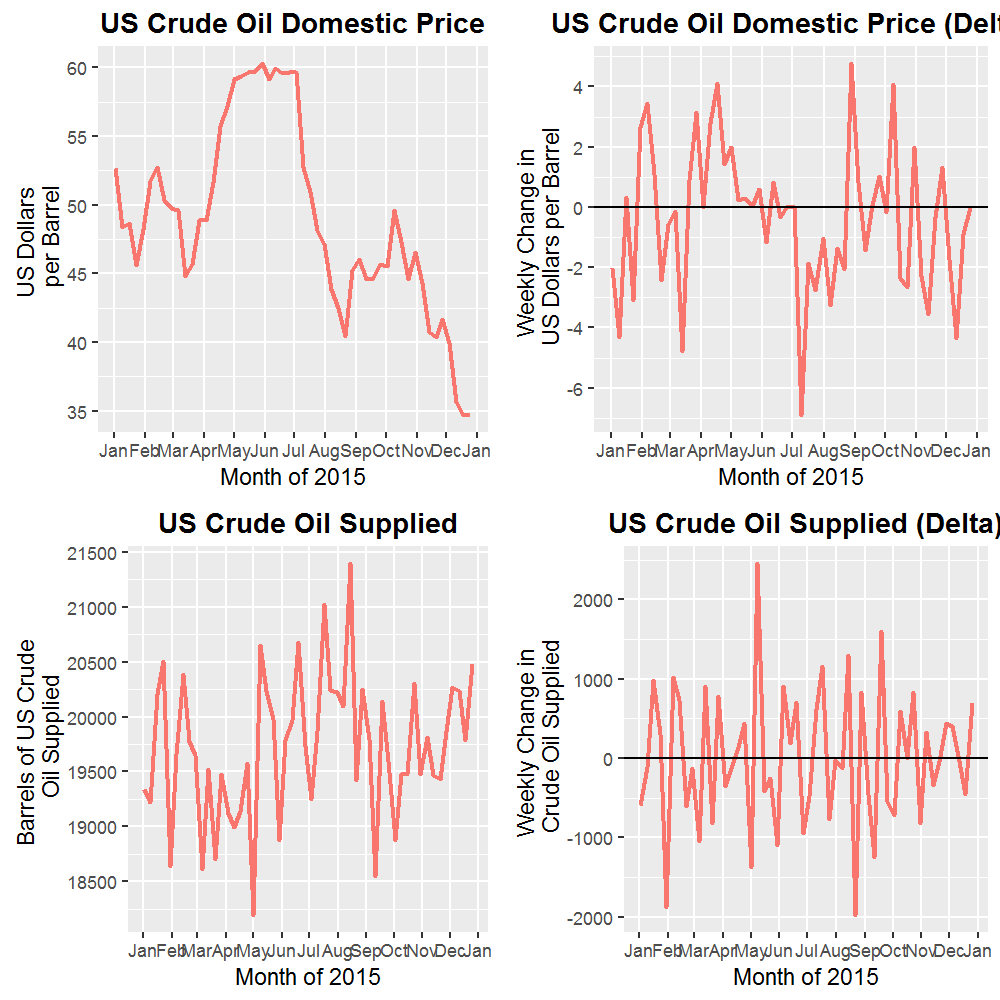
\includegraphics[height=10.41667in]{images/EIAdata_us_crudeoil_pricesupply.png}

\newpage

\subsection{Figure B8 U.S. Crude Oil Price Decomposition
Plot}\label{figure-b8-u.s.-crude-oil-price-decomposition-plot}

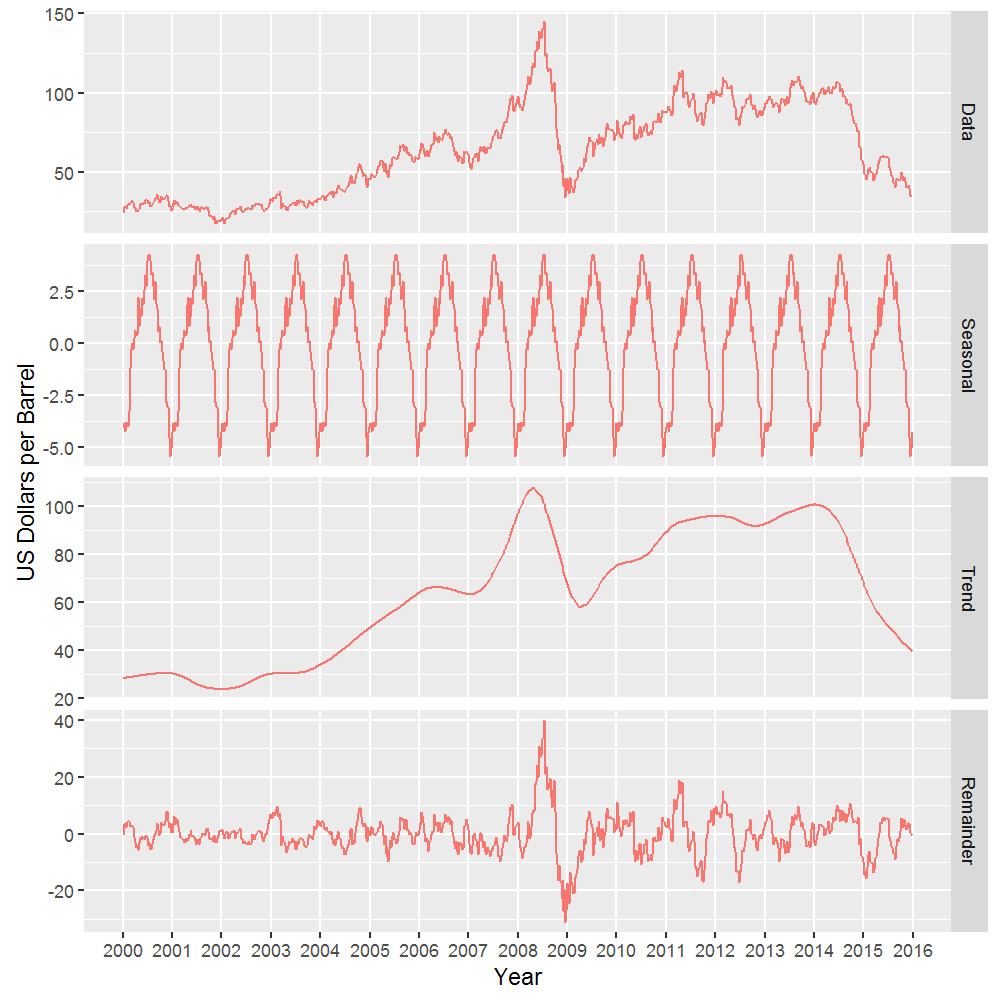
\includegraphics[height=10.41667in]{images/EIAdata_us_crudeoil_pricedecomp.png}

\newpage

\subsection{Figure B9 U.S. Crude Oil Price
Forecast}\label{figure-b9-u.s.-crude-oil-price-forecast}

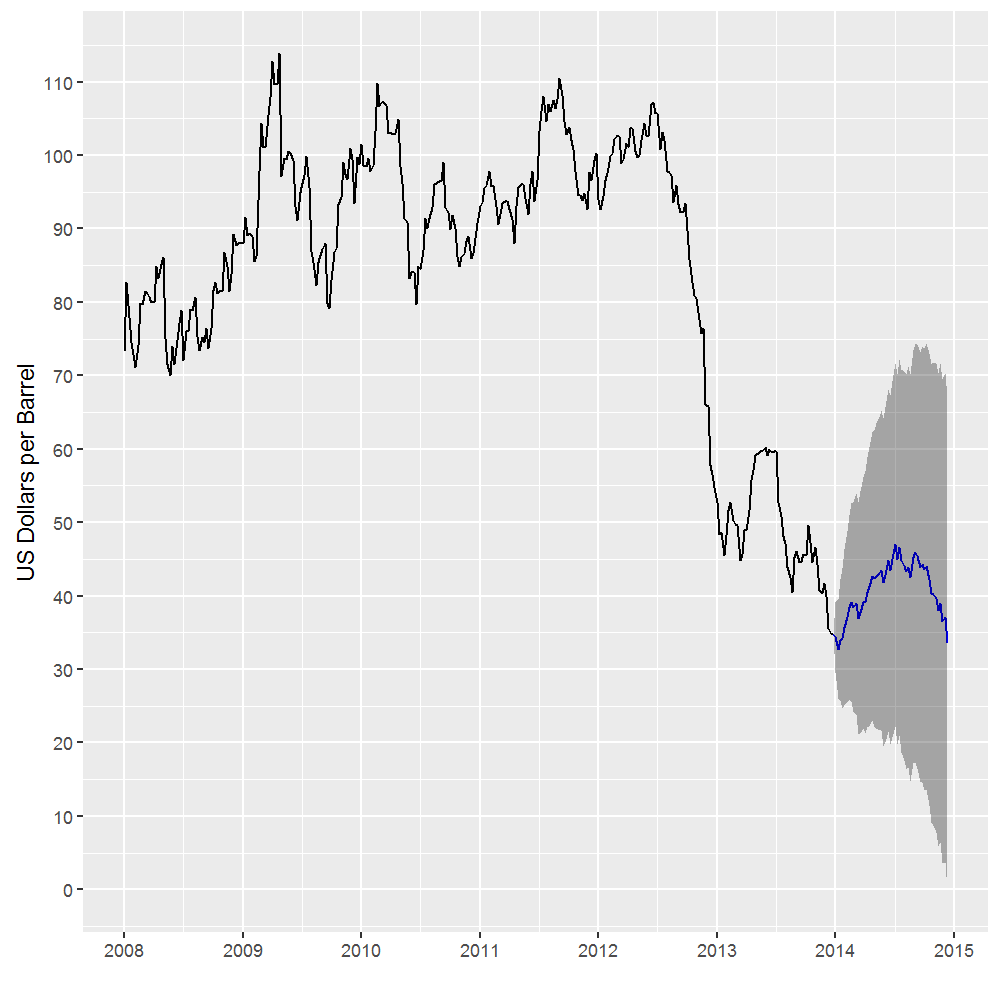
\includegraphics[height=10.41667in]{images/EIAdata_us_crudeoil_priceforecast.png}

\newpage

\section*{References}\label{references}
\addcontentsline{toc}{section}{References}

\hypertarget{refs}{}
\hypertarget{ref-eia}{}
Agency, Energy Information. 2016. ``EIA: Energy Information Agency.''
\url{http://www.eia.gov}.

\hypertarget{ref-Baff2015}{}
J. Baffes, F. Ohnsorge, M. Ayhan Kose. 2015. ``Down the Slide.''
\url{http://www.imf.org/external/pubs/ft/fandd/2015/12/baffes.htm}.

\hypertarget{ref-Saun2015}{}
Saunders, T. 2015. ``Developments in Thermal Coal Markets.''
\url{http://www.rba.gov.au/publications/bulletin/2015/jun/pdf/bu-0615-3.pdf}.


\end{document}
